\begin{ledgroupsized}[r]{120mm}
\footnotesize
\pstart%
\noindent\textbf{\"{U}berlieferung:}%
\pend
\end{ledgroupsized}
%
\begin{ledgroupsized}[r]{114mm}
\footnotesize%
\pstart%
\parindent -6mm%
\makebox[6mm][l]{\textit{L}}%
Konzept: LH XXXV 14, 2 Bl. 51. 1 Bl. 8\textsuperscript{o}. 1 S. auf Bl. 51~r\textsuperscript{o}.
Auf Bl. 51~v\textsuperscript{o} finden sich 2 Z. von Schreiberhand mit einer \"{U}berschrift aus den \textit{Digesta Iustiniani}, lib. VII, cap. 5:
\textit{Tit. V. De usufructu earum rerum quae usu consumuntur vel minuuntur.}\\%
Cc2, Nr. 00.
\pend
\end{ledgroupsized}
%\normalsize
\vspace*{5mm}
\begin{ledgroup}
\footnotesize%
\pstart%
\noindent%
\footnotesize{\textbf{Datierungsgr\"{u}nde:}
Die \"{U}berschrift auf der R\"{u}ckseite legt die Vermutung nahe, dass es sich um Papier für das \title{Corpus juris reconcinnatum} handelt (siehe hierzu \textit{LSB} VI, 2, S. XXIf.). Das St\"{u}ck d\"{u}rfte daher in der Mainzer Zeit nach Beginn der Arbeiten am \textit{CJR} entstanden sein.}
\pend
\end{ledgroup}
%
\vspace*{8mm}
\pstart%
\noindent%
\normalsize%
%[51~r\textsuperscript{o}]
% 
\begin{wrapfigure}{l}{0.25\textwidth}                    
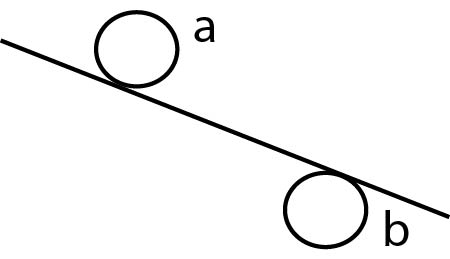
\includegraphics[width=0.25\textwidth]{images/lh0351402_51-d.pdf}\\
\rule[0cm]{14mm}{0cm}[\textit{Fig. 1}]\\                       
%\caption{Bildbeschreibung}
\end{wrapfigure}
Concursus Gravitatis duplicis \edtext{unius}{\lemma{duplicis}\Bfootnote{ \textit{ (1) }\ tum \textit{ (2) }\ unius \textit{ L }\ }} Liberae\protect\index{Sachverzeichnis}{libra}, alterius in plano inclinato experimentum capi potest. Si grave\protect\index{Sachverzeichnis}{grave} sit liquidum, ut gutta aquae aut cerae\protect\index{Sachverzeichnis}{cera} liquefactae in plani inclinati\protect\index{Sachverzeichnis}{planum inclinatum} superficie inferiore decurrens. Id est non in \textit{a.} sed in \textit{b.}
\edtext{Sume}{\lemma{$b.$}\Bfootnote{ \textit{ (1) }\ ita enim \textit{ (2) }\ Sume \textit{ L }\ }} candelam\protect\index{Sachverzeichnis}{candela} ardentem hanc oblique tene et observa \edtext{quanta}{\lemma{observa}\Bfootnote{ \textit{ (1) }\ quousque \textit{ (2) }\ quanta \textit{ L }\ }} maxima obliquitate defluat gutta potius in candela, quam delabatur in pavimentum. Fateor tamen gravitatem\protect\index{Sachverzeichnis}{gravitas} tenacitate\protect\index{Sachverzeichnis}{tenacitas} massae\protect\index{Sachverzeichnis}{massa} adjuvari, sed etsi massa utcunque liquida sit ut in gutta aquae aut Mercurij\protect\index{Sachverzeichnis}{mercurium} aliquamdiu tamen etiam ex plano horizonti parallelo pendere constat, ut in tabulis planis laevigatis sibi impositis fieri videmus.
Caeterum hoc experimento aestimari possunt tenacitatis gradus.
\pend
\pstart%
Novum cristallisationis\protect\index{Sachverzeichnis}{cristallisatio} genus si aquam in qua sal aliquod solutum \edtext{spissiorem}{\lemma{solutum}\Bfootnote{ \textit{ (1) }\ est \textit{ (2) }\ spissiorem \textit{ L }\ }} reddas non\edtext{}{\lemma{}\Bfootnote{non  \textbar\ aquae \textit{ gestr.}\ \textbar\ decoctione \textit{ L }\ }} decoctione, sed compressione. Ita enim spes est cristallos\protect\index{Sachverzeichnis}{cristallus} nihilo minus micaturas.
\pend